% -*- root: ../Economia.tex -*-
\section{Modelos de un período}
\begin{problem}[1]
El subyacente $S$ vale hoy 60 \texteuro y el modelo que hemos definido prevé, para el tiempo siguiente, un nivel alto en 65 \texteuro y un nivel bajo en 55 \texteuro. El tipo libre de riesgo para el período es del 3\%.
\ppart Calcular la probabilidad riesgo neutro del estado alto de la economía.
\ppart Calcular el valor de una put con precio de ejercicio en 60 \texteuro.
\ppart Misma pregunta si el tipo libre de riesgo, para la composición continua, es ahora del 6\% y el tiempo hasta vencimiento es de seis meses.

\solution

\spart

La situación que descibe el problema puede representarse mediante el siguiente diagrama:

\begin{minipage}{0.48\textwidth}
\begin{center}
\begin{tikzpicture}[->,>=stealth',shorten >=1pt,auto,node distance=2.8cm,
                    semithick]
  %\tikzstyle{every state}=[fill=red,draw=none,text=white]

  \node[state] (A)                    {$S_0$};
  \node[state] (B) [above right of=A] {$aS_0$};
  \node[state] (C) [below right of=A] {$bS_0$};


  \path (A) edge node {q} (B)
  		    edge node {1-q} (C);
\end{tikzpicture}
\end{center}
\end{minipage}
\begin{minipage}{0.48\textwidth}
Siendo en este caso concreto
\[\begin{array}{l}
S_0 = 60 \\
aS_0 = 65 \implies a = 1.08 \\
bS_0 = 55 \implies b = 0.92
\end{array}\]
\end{minipage}

Lo primero que debemos hacer es calcular la probabilidad riesgo neutro, que es aquella que hace que se cumpla la conidición de martingala.

La condición de martingala se escribe como:
\[V_0(\varphi) = \tilde{V}_0(\varphi) = \esp[Q]{\tilde{V}_1(\varphi)}\]

Vamos a forzar que se cumpla esta conidción para despejar el valor de $q$ que buscamos. Para ello suponemos la estrategia trivial $\varphi=(\varphi_1) =(1)$.

\[\esp[Q]{\tilde{V}_1(\varphi)} = \frac{q\cdot aS_0 + (1-q)\cdot bS_0}{S_1^0} = \frac{65q + (1-q)55}{1+r} = \frac{10q+55}{1.03}\]

Por otro lado sabemos que $V_0(\varphi) = 60$ con lo que igualando llegamos a:
\[\frac{10q+55}{1.03} = 60 \implies 10q = 6.8 \implies q = 0.68 \]

\spart

Una \concept{put} es un contrato que da el derecho a vender en tiempo $t=1$ una acción de $S$ por $K$ euros.

Suponiendo que no hubiera ningún tipo de tasa ni impuesto extra que pagar (suposición que no es cierta en los mercados reales) el precio o coste de una put puede calcularse como su valor en el instante $t=0$.

Teniendo los mismos estados del apartado anterior con sus mismos valores y siendo el precio de ejercicio $K=60$ \texteuro (el precio al que garantizamos vender en el futuro) podemos ver que en el estado alto tenemos un valor $X(ω_1)=0$\footnote{Tengo derecho a vender a $K$ pero ha subido y la podré vender a más de $K$, por tanto no ejerceremos la put} y en el caso bajo $X(ω_2)=K-bS_0$\footnote{Lo que gano es la diferencia entre el precio al que habría vendido sin la put y el precio a que vendo gracias a ella}.

Conociendo la probabilidade riesgo neutra, que calculamos en el aprtado anterior, podemos calcular el valor inicial de la put con la misma fórmula usada en el apartado anterior:
\[P_0 = V_0(\varphi) = \tilde{V}_0(\varphi) = \esp[Q]{\tilde{V}_1(\varphi)} = (1-q) \frac{K-bS_0}{1+r} = 0.32 \cdot \frac{60-55}{1.03}=1.55\]

\spart

Hasta ahora lo que hemos visto es que tenemos un tipo de interes simple que consiste en que nos perstan una cantidad $X$ con un interés $r$ y al final del ejercicio devolvemos la cantidad prestada más los intereses, es decir, ent $t=1$ pagamos
\[(1+r)X\]

No obstante, podríamos considerar que en el instante $t=1/2$ pagamos los intereses correspondientes a 6 meses y en $t=1$ pagamos los intereses de los segundos 6 meses y, además, devolvemos todo el préstamos inicial. En esta ocasión estaríamos pagando
\[\left(1+\frac{r}{2}\right)^2\]

En general, si dividimos los pagos en $n$ plazos estamos pagando
\[\left( 1 + \frac{r}{n} \right)^n\]

Es sencillo ver que si extendemos esta distribución de préstamos hasta considerar intervalos infinitamente pequeños llegamos a una \concept{composición continua} donde la función que mide lo que debemos pagar se corresponde con una exponencial. Es decir, tendiendo $n$ al infinito lo que estamos pagando es:
\[e^{rt}\cdot X\]

Por tanto, lo único que debemos hacer para trabajar en este tipo de casos es sutituir las operaciones que realizábamos con respecto a $1+r$ al trabajar con precios descontados por las mismas operaciones respecto a $e^{rt}$.

Puesto que estamos considerando vencimiento de 6 meses tendremos:
\[P_0 = V_0(\varphi) = \tilde{V}_0(\varphi) = \esp[Q]{\tilde{V}_1(\varphi)} = (1-q) \frac{K-bS_0}{e^{rt}} = 0.32 \cdot \frac{60-55}{e^{0.06\cdot 0.5}}=1.55\]
\end{problem}

\begin{problem}[2]
El subyacente $S$ vale hoy 10 \texteuro y el model definido prevé, para el tiempo siguiente, un nivel alto en 12 \texteuro y un nivel bajo en 9 \texteuro. El tipo libre de riesgo para el período es del 10\%. Consideramos un derivado $X$ que pagará el cuadrado del valor $S_1$ a vencimineto.

\ppart ¿Cuál es la cartera de cobertura para dicho derivado?
\ppart Calcular el valor de dicho derivado en 0.
\ppart Calcular el valor de una call sobre este derivado con un precio de ejercicio de 100.
\ppart Un segundo análisis le lleva a pensar que los dos estados futuros del modelo han de ser 10.5 y 9.5 (permaneciendo inalterado el tipo libre de riesgo). ¿Es el nuevo modelo viable (libre de arbitrajes)? [Intenta calcular la probabilidad riesgo neutro del estado alto]

\solution

\spart

La \concept{cartera de cobertura} no es más que aquella que a vencimiento nos garantiza los mismos resultados que el derivado que queremos cubrir.

Tenemos por ahora un derivado $S^0$ que es la \concept{cuenta bancaria} que tiene un interés fijo y conocido; y el activo descrito por el enunciado, $S$, que llamaremos $S^1$ que sigue el siguiente esquema

\begin{minipage}{0.48\textwidth}
\begin{center}
\begin{tikzpicture}[->,>=stealth',shorten >=1pt,auto,node distance=2.8cm,
                    semithick]
  %\tikzstyle{every state}=[fill=red,draw=none,text=white]

  \node[state] (A)                    {$S_0^1$};
  \node[state] (B) [above right of=A] {$aS_0^1$};
  \node[state] (C) [below right of=A] {$bS_0^1$};


  \path (A) edge node {q} (B)
  		    edge node {1-q} (C);
\end{tikzpicture}
\end{center}
\end{minipage}
\begin{minipage}{0.48\textwidth}
Siendo en este caso concreto
\[\begin{array}{l}
S_0^1 = 10 \\
aS_0^1 = 12 \implies a = 1.2 \\
bS_0^1 = 9 \implies b = 0.9
\end{array}\]
\end{minipage}

La estrategia de cobertura será aquella $\varphi=(\varphi_0,\varphi_1)$ compuesta por los activos $S^0$ y $S^1$ que, a vencimiento, nos da los mismos resultados que el activo $X$. Para encontrar esta cartera simplemente debemos resolver la ecuación:
\[\left\{ \begin{array}{l}
\varphi_0\cdot 1.1 + \varphi_1\cdot 12 = 144 \\
\varphi_0\cdot 1.1 + \varphi_1\cdot 9 = 81
\end{array}\right. \implies \varphi_1 = 21 \text{ y } \varphi_0 = -98.18\]

\spart

Para conocer el valor de este derivado en $t=0$ necesitamos conocer cuál es la probabilidad de que se de cada suceso de los planteados para $t=1$.

Vamos a centrarnos en el activo $S^1$ que conocemos. Puesto que \textbf{suponemos que estamos trabajando en una economía libre de arbitrajes} sabemos que existe la \concept{probabilidad riesgo neutro}, que es aquella que garantiza que el valor de precios descontados de una cartera coincida con su valor inicial. Es decir:
\[V_0(\varphi) = \tilde{V}_0(\varphi) = \esp[Q]{\tilde{V}_1(\varphi)}\]

Por tanto, para conocer esta probabilidad sólamente tenemos que resolver la ecuación:
\[10 =  \frac{q\cdot aS_0 + (1-q)\cdot bS_0}{S_1^0} =  \frac{q\cdot 12 + (1-q)\cdot 9}{1.1} = \frac{3q + 9}{1.1} \implies q=0.67\]

Una vez conocemos esta probabilidad, podemos calcular el valor del derivado como valor descontado esperado del mismo:
\[V_0(X) = \frac{qX(ω_1) + (1-q)X(ω_2)}{1+r} = \frac{0.67\cdot 144 + 0.33\cdot 81}{1.1} = 112\]

\spart

Una \concept{call} es un contrato que da derecho a comprar un producto $S$ por $K$ euros en tiempo $t=1$.

En esta ocasión tenemos un precio $K=100$ \texteuro. Para calcular su precio lo único que debemos hacer es considerarlo como un derivado más y aplicar el mismo razonamiento que empleamos al final del apartado anterior.

Con probabilidad $q$ estaremos en el estado alto, por lo que compraremos el derivado de precio 144 \texteuro por los 100 \texteuro acordados en la call, con lo que ganamos 44 \texteuro. Por otro lado, si estamos en el estado bajo de la economía, optamos por no comprar con lo que no perdemos nada. Por tanto tenemos $X(ω_1)=aS^1_0-K$ y $X(ω_2)=0$. Así tenemos:

\[C_0 = \frac{qX(ω_1) + (1-q)X(ω_2)}{1+r} = \frac{0.67(144-100)}{1.1} = 26.8\]

\spart

Con la nueva situación descrita, y siguiendo la indicación del enunciado, tratamos de calcular la probabilidad riesgo neutro correspondiente. Así tenemos:
\[10 = \frac{10.5q + (1-q)9.5}{1+r} = \frac{q+9.5}{1.1}\implies q=1.5 \]

Evidentemente esta situación no es posible puesto que $q$ es una probabilidad, que no puede ser mayor que 1. Veamos cómo estudiar esta situación.

Si nos fijamos podemos observar que en el estado alto de este activo tenemos un valor menor que el correspondiente a la cuenta bancaria. Aquí surge el \concept{arbitraje}: nos ponemos en corto con el activo $S$, es decir, vendemos $n$ acciones de $S$ que aún no hemos comprado. El dinero ganado con esta puesta en corto, $10\cdot n$ \texteuro, lo metemos en una cuenta bancaria con tipo libre de riesgo $1.1$.

En $t=1$ debemos comprar las acciones de $S$ al precio que estén para entregarlas que seguro será menor que la cantidad que tenemos en el banco. Por tanto, \textbf{estamos ganando dinero sin riesgo alguno}.
\end{problem}

\begin{problem}[3]
El subyacente $S$ vale hoy 10 \texteuro y el modelo que hemos definido prevé, para el tiempo siguiente, un nivel alto en 12 \texteuro y un nivel bajo en 8 \texteuro. El tipo libre de riesgo para el período es del 5\%. Calcular el valor de una call de precio de ejercicio 11 \texteuro:
\ppart Por no arbitraje

\ppart Por valoración riesgo neutro.
\solution

Empezamos calculando la probabilidad riesgo neutro asociada al estado alto de este modelo. Nuevamente, reutilizamos las fórmulas y los conceptos de los dos ejercicios anteriores. Así tenemos
\[10 = \frac{12q + (1-q)8}{1.05} = \frac{4q+8}{1.05} \implies q=0.63\]

\spart

Vamos a buscar la estrategia de cobertura de este activo que es la call. Así tenemos que resolver el siguiente sistema:

\[\left\{ \begin{array}{l}
\varphi_0 \cdot 1.05 + \varphi_1\cdot 12 = 1 \\
\varphi_0 \cdot 1.05 + \varphi_1\cdot 8 = 0
\end{array}\right. \implies \varphi_1 = 0.25 \text{ y } \varphi_0 = -1.9\]

Puesto que estamos bajo la suposición de que nos movemos en una economía libre de arbitrajes, el precio inicial de esta estrategia debe coincidir con el previo actual del activo $X$ (la réplica de la call).

Así tenemos:
\[C_0 = V_0(\varphi) = \varphi_1 S_0^1 + \varphi_0S_0^0 = 0.25 \cdot 10 - 1.9 = 0.6\]
\spart

Una vez conocemos la probabilidad riesgo neutro podemos calcular el precio de la call como sigue:
\[C_0 = q\cdot \frac{aS_0 - K}{1+r} = 0.63 \frac{12-11}{1.05} = 0.6\]

Como era de esperar los dos procedimientos nos llevan a la obtención del mismo precio.
\end{problem}

\begin{problem}[4]
La ausencia de oportunidades de arbitraje es una de las exigencias más fuertes que se le pueden hacer al modelo. Una exigencia primera es la ley de un único precio: el modelo no puede asignar dos precios distintos a un mismo subyacente o derivado por una cuestión elemental de consistencia.

\ppart Comprobar que un modelo con $S_0 = 10$ y $S_1(ω_1)=S_1(ω_2)=12$ no satisface la ley de único precio, siendo $r=0.1$.
% Comenté este ejercicio con el profesor y concluimos que era necesario un valor de r que no proporciona el enunciado. Nos inventamos un valor que tuviera sentido.

\ppart ¿Puede dar otro ejemplo?
\solution

\spart
Considerando el activo $S$ descrito en el enunciado, vamos a comprobar cuál es el precio actual de ese activo, atendiendo a sus precios de futuro tanto en el estado alto como en el bajo.

\[S_0 = \frac{qS_1(ω_1) + (1-q)S_1(ω_2)}{1+r} = \frac{12}{1.1}=10.9\]

Es evidente comprobar que este precio inicial no se corresponde con $S_0=10$ por lo que la ley de único precio no se satisface.

\spart

Apoyándonos en el ejercicio anterior, es sencillo ver que el siguiente modelo no cumple la ley de precio único.
\[\left\{\begin{array}{l}
C_0 = 1 \\
K = 11 \\
r = 0.05\\
S_0 = 10 \\
S_1(ω_1) = 12\\
S_2(ω_2) = 8
\end{array}\right.\]


\end{problem}

\begin{problem}[5]
Se dice que una estrategia $\tilde{\varphi}$ domina a otra estrategia $\varphi$ $(\varphi \prec \tilde{\varphi})$ si $V_0=\tilde{V}_0$ y $V_1(w) < \tilde{V}_1(ω)$ para todo $ω \in Ω$.

\ppart Comprobar que en un modelo con $S_0=10$ y $S_1(ω_1)=12$ y $S_1(ω_2) = 8$ con $r=1$ $\varphi=(10,-1)$ es una estrategia dominante,

\ppart Demostrar, sin embargo, que se cumple la ley de un precio.

\ppart Construir un arbitraje
\solution

\spart
\doneby{Pedro}

La estrategia $\varphi = (10,-1)$ tiene un valor inicial:
\[V_0(\varphi)=10-1\cdot 10 = 0\]

Para garantizar que la estrategia es dominante debemos comprobar que cualquier otra estrategia con valor inicial 0 tiene valores finales (tanto en el estado alto como en el bajo) menores que $V_1(\varphi(ω))$.

Dados los activos con los que estamos trabajando (la cuenta sin riesgo y $S$), toda estrategia que tenga valor 0 en $t=0$ será de la forma:
\[\varphi_a = (10a, -a) \text{ con } a \in \ent\]

Para la estrategia dada por el enunciado tenemos:
\[\left\{ \begin{array}{l}
V_1(\varphi(ω_1))= 10(1+r) -12  = 8\\
V_1(\varphi(ω_2))= 10(1+r) - 8 = 12
\end{array}\right.\]

Por otro lado, para una estrategia $\varphi_a$ cualquiera tendremos:
\[\left\{ \begin{array}{l}
V_1(\varphi_a(ω_1))= a\cdot 10(1+r) -a\cdot 12  = a\cdot 8\\
V_1(\varphi_a(ω_2))= a\cdot 10(1+r) - a\cdot 8 = a\cdot 12
\end{array}\right.\]

A priori parece sencillo comprobar que la estrategia no es dominante puesto que según el valor de $a$ podemos tener un valor final más alto para $\varphi_1$ que para $\varphi$.

Sin embargo, siempre que tengamos una estrategia con valor final positivo tanto en el estado alto como en el bajo, los múltiplos de esta estrategia tendrán mayores valores a vencimiento. Por tanto parece lógico considerar, aunque no lo diga el enunciado como tal, que la definición dominancia se refiere a estrategias que no son múltiplo de la dada.

Con esta última asunción queda claro que la estrategia dada es dominante pueso que no existe otra estrategia de valor $0$ (mas allá de la trivial de no comprar nada, que tiene valor a vencimiento $0$)

\spart



\end{problem}

\begin{problem}[6]
Consideremos ahora el modelo con $S_0=10$ y $S_1(ω_1)=12$ y $S_1(ω_2)=10$ con $r=0$.

\ppart Construir un arbitraje
\ppart Demostrar que bajo la probabilidad definida por $Q(ω_1)=0$ y $Q(ω_2)=1$ el proceso de precios descontados es una martingala.
\ppart Deducir de ello que no hay estrategias dominantes
\ppart Explicar la aparente contradicción entre los apartados a) y b)
\solution
\doneby{Pedro}

\spart

Recordemos que un arbitraje no era más que la posibilidad de ganar dinero sin arriesgar. En este caso la estrategia $\varphi=(0,1)$ ya constituye un arbitraje pues ganamos 2 con probabilidad $q$ y nos quedamos como estamos en caso contrario.

\spart

Para que el proceso de precios descontados sea una martingala necesitamos que:
\[V_0(\varphi) = \esp[q]{\tilde{V}_1(\varphi)}\equiv \varphi_0+10\varphi_1 = (\varphi_0+12\varphi_1)Q(ω_1) + (\varphi_0 +10\cdot  \varphi_1)Q(ω_2)\]
siendo $\varphi_i$ la cantidad de acciones del activo $S^i$

que es obviamente cierto puesto que $Q(w_1)=0$ y $Q(ω_2)=1$.

\spart

\spart

El apartado b) está cambiando el modelo en el que trabajamos puesto que dejamos de tener dos estados en $t=1$ para tener sólo 1, puesto que la probabilidad de uno de ellos es 0.

\end{problem}


\begin{problem}[7]
El economista francés Maurice Allais ha sido uno de los primeros en describir situaciones en las cuales el comportamiento de los agentes no es racional. Después de esto, todo un área, el de las \textbf{finanzas comportamentales}, se ha ido desarrollando y consolidando. Consideremos las dos situaciones siguientes:

\begin{enumerate}
\item Un grupo de individuos recibe 1000  y debe elegir una de las dos loterías siguientes:
\begin{enumerate}
\item[a)] Una ganancia segura de 500
\item[b)] Una lotería que tiene probabilidad 0.5 de dar 1000 y 0.5 de dar 0.
\end{enumerate}

\item Un grupo de individuos recibe 2000 y debe elegir una de las dos loterías siguientes:
\begin{enumerate}
\item[a)] Una pérdida segura de 500
\item[b)] Una lotería que tiene probabilidad 0.5 de perder 1000 y 0.5 de perder 0.
\end{enumerate}
\end{enumerate}

\ppart Comprobar que, dadas las condiciones iniciales, ambas loterías conducen a los mismos resultados.

Como curiosidad, cabe destacar que por lo general la gente opta por la opción a) en el primer caso y por la opción b) en el segundo.
\solution

Para empezar podemos ver que la esperanza de las cuatro diferentes opciones es la misma.

\[\begin{array}{l}
\esp{X_{1a}} = 1000 + 500 = 1500\\
\esp{X_{1b}} = 1000 + 0.5\cdot 1000 + 0.5 \cdot 0 = 1500 \\
\esp{X_{2a}} = 2000 - 500 = 1500 \\
\esp{X_{2b}} = 2000 - 0.5 \cdot 1000 - 0.5 \cdot 0 = 1500
\end{array}\]

\end{problem}

\section{Árboles binomiales}

\begin{problem}[1]
El subyacente $S$ vale hoy 10 y su dinámica está descrita por un árbol binomial recombinante de cuatro periodos a un horizonte temporal de 6 meses. La volatilidad del subyacente es del 25\% y el tipo libre de riesgo para el periodo es del 5.5 \% (composición continua)

\ppart Calcular la \textbf{call look back} cuyo flujo final es $S_4-\min\{S_i/ i\leq 4\}$.

\ppart Misma pregunta para la \textbf{put lookback} cuyo flujo final es $\max\{S_i / i \leq 4\}-S_4$.
\solution

\doneby{Pedro}

Los datos que conocemos nada más leer el enunciado son:
\[S_0=10, \ T=0.5, \ Δt = 0.125, \ σ=0.25, \ R_c=0.055\]

El arbol binomial en esta situación es:
\begin{center}
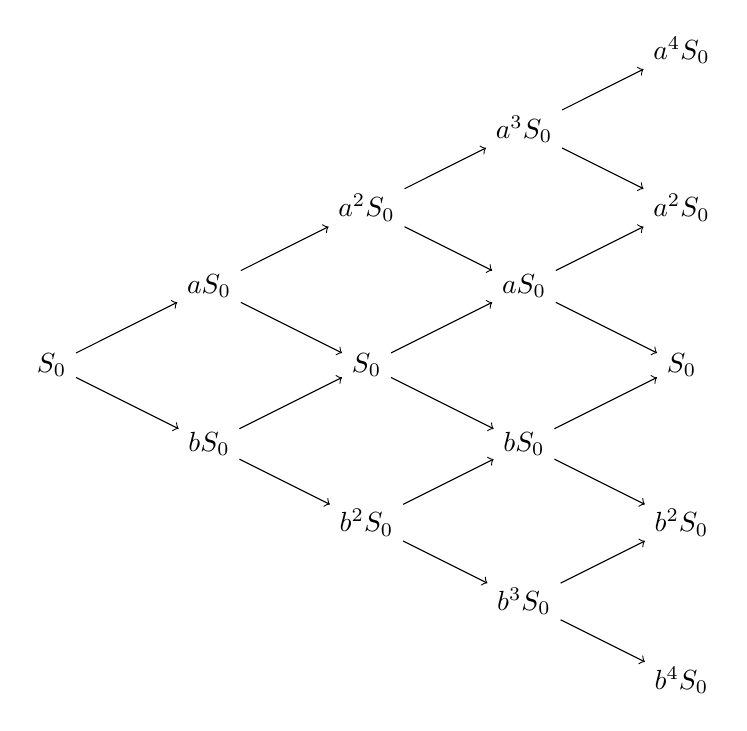
\begin{tikzpicture}
[   cnode/.style={draw=black,fill=#1,minimum width=3mm,circle},
]
\node[] (A) at (0,0) {$S_0$};
\node[] (B) at (2,1) {$aS_0$};
\node[] (C) at (2,-1) {$bS_0$};
\node[] (D) at (4,2) {$a^2S_0$};
\node[] (E) at (4,0) {$S_0$};
\node[] (F) at (4,-2) {$b^2S_0$};
\node[] (G) at (6,3) {$a^3S_0 $};
\node[] (H) at (6,1) {$aS_0 $};
\node[] (I) at (6,-1) {$bS_0 $};
\node[] (J) at (6,-3) {$b^3S_0 $};
\node[] (K) at (8,4) {$a^4S_0$};
\node[] (L) at (8,2) {$a^2S_0$};
\node[] (M) at (8,0) {$S_0$};
\node[] (N) at (8,-2) {$b^2S_0$};
\node[] (O) at (8,-4) {$b^4S_0$};

\draw[->] (A) -- (B);
\draw[->] (A) -- (C);
\draw[->] (B) -- (D);
\draw[->] (B) -- (E);
\draw[->] (C) -- (E);
\draw[->] (C) -- (F);
\draw[->] (D) -- (G);
\draw[->] (D) -- (H);
\draw[->] (E) -- (H);
\draw[->] (E) -- (I);
\draw[->] (F) -- (I);
\draw[->] (F) -- (J);
\draw[->] (G) -- (K);
\draw[->] (G) -- (L);
\draw[->] (H) -- (L);
\draw[->] (H) -- (M);
\draw[->] (I) -- (M);
\draw[->] (I) -- (N);
\draw[->] (J) -- (N);
\draw[->] (J) -- (O);


\end{tikzpicture}
\end{center}

Con los datos del enunciado podemos calcular los valores de $a$ y $b$ mostrados en el esquema, así como la probabilidad de que se de cada suceso. Tomando las fórmulas vistas en los apuntes tenemos:
\[a=e^{σ\sqrt{Δt}} = 1.09, \ b = \frac{1}{a} = 0.92, \ p = \frac{e^{r_cΔt}-b}{a-b}=0.52\]

\spart
Puesto que el valor de la call descrita en el enunciado depende del camino seguido, debemos considerar los 16 posibles caminos para estudiar, en cada caso, cuál es el valor final del activo. La siguiente tabla recoge los resultados obtenidos:

\begin{center}
\begin{tabular}{|c|c|c|c|}
\hline
\textbf{Trayectoria} & \textbf{Probabilidad} & \textbf{Valor del activo} & \textbf{Valor del derivado}\\
\hline
aaaa & $p^4$        & $a^4S_0$ & $a^4S_0-S_0$ \\
aaab & $p^3(1-p)$   & $a^2S_0$ & $a^2S_0-S_0$ \\
aaba & $p^3(1-p)$   & $a^2S_0$ & $a^2S_0-S_0$ \\
aabb & $p^2(1-p)^2$ & $S_0$ & $0$ \\
abaa & $p^3(1-p)$   & $a^2S_0$ & $a^2S_0-S_0$ \\
abab & $p^2(1-p)^2$ & $S_0$ & $0$ \\
abba & $p^2(1-p)^2$ & $S_0$ & $S_0-bS_0$ \\
abbb & $p(1-p)^3$   & $b^2S_0$ & $0$ \\
baaa & $p^3(1-p)$   & $a^2S_0$ & $a^2S_0-bS_0$ \\
baab & $p^2(1-p)^2$ & $S_0$ & $S_0-bS_0$ \\
baba & $p^2(1-p)^2$ & $S_0$ & $S_0-bS_0$ \\
babb & $p(1-p)^3$   & $b^2S_0$ & $0$ \\
bbaa & $p^2(1-p)^2$ & $S_0$ & $S_0-b^2S_0$ \\
bbab & $p(1-p)^3$   & $b^2S_0$ & $0$ \\
bbba & $p(1-p)^3$   & $b^2S_0$ & $b^2S_0-b^3S_0$ \\
bbbb & $(1-p)^4$    & $b^4S_0$ & $0$ \\
\hline
\end{tabular}
\end{center}

Para calcular el valor futuro de este activo simplemente tenemos que multiplicar el valor del derivado por la probabilidad de alcanzar ese valor y sumar los resultados.

Con un script de python, que puede encontrarse en el apéndice \ref{sec:arbolBin}, calculamos el valor de este activo en el instante final y obtenemos:
\[V_T(X) = 1.18\]

Una vez tenemos este valor, podemos traerlo al presente dividiendo entre $e^{r_cΔtn}$, que en este caso sería $e^{0.055\cdot 0.5}$, con lo que obtenemos:
\[V_0(X) = 1.14\]

\spart

Con el mismo razonamiento del apartado anterior tenemos:

\begin{center}
\begin{tabular}{|c|c|c|c|}
\hline
\textbf{Trayectoria} & \textbf{Probabilidad} & \textbf{Valor del activo} & \textbf{Valor del derivado}\\
\hline
aaaa & $p^4$        & $a^4S_0$ & $0$ \\
aaab & $p^3(1-p)$   & $a^2S_0$ & $a^3S_0-a^2S_0$ \\
aaba & $p^3(1-p)$   & $a^2S_0$ & $0$ \\
aabb & $p^2(1-p)^2$ & $S_0$ & $a^2S_0-S_0$ \\
abaa & $p^3(1-p)$   & $a^2S_0$ & $0$ \\
abab & $p^2(1-p)^2$ & $S_0$ & $aS_0-S_0$ \\
abba & $p^2(1-p)^2$ & $S_0$ & $aS_0-S_0$ \\
abbb & $p(1-p)^3$   & $b^2S_0$ & $aS_0-b^2S_0$ \\
baaa & $p^3(1-p)$   & $a^2S_0$ & $0$ \\
baab & $p^2(1-p)^2$ & $S_0$ & $aS_0-S_0$ \\
baba & $p^2(1-p)^2$ & $S_0$ & $0$ \\
babb & $p(1-p)^3$   & $b^2S_0$ & $S_0-b^2S_0$ \\
bbaa & $p^2(1-p)^2$ & $S_0$ & $0$ \\
bbab & $p(1-p)^3$   & $b^2S_0$ & $S_0-b^2S_0$ \\
bbba & $p(1-p)^3$   & $b^2S_0$ & $S_0-b^2S_0$ \\
bbbb & $(1-p)^4$    & $b^4S_0$ & $S_0-b^4S_0$ \\
\hline
\end{tabular}
\end{center}

A partir de esta tabla podemos calcular sin problema el valor futuro del derivado combinando la segunda y la cuarta columna. Una vez tenemos esto, como en el apartado anterior, simplemente lo traemos al presente multiplicando por $e^{-0.055\cdot 0.5}$

Empleando de nuevo el script \ref{sec:arbolBin} tenemos:
\[V_T(X) = 0.90 \implies V_0(X) = 0.88\]
\end{problem}

\begin{problem}[2]
Consideramos un subyacente $S$ que vale hoy 12 y cuya dinámica está descrita por un árbol binomial recombinante de 10 períodos mensuales. La volatilidad del subyacente es del 25\% y el tipo libre de riesgo para el periodo es del 3.5 \% (composición continua). Sea $a$ el coeficiente correspondiente del árbol binomial.

\ppart Calcular el valor de una call europea con una barrrera up-and-out en el nivel $a^8S_0$.
\ppart ¿Qué se puede decir de la opción barrera up-and-in de similares características?
\ppart Calcular el valor de una put europea con una barrera down-and-out en el nivel $a^{-8}S_0$.
\ppart ¿Qué se puede decir de una opción barrera down-and-in de similares características?
\ppart Calcular el precio de una opción barrera digital que paga $1$ a vencimiento si la barrera ha sido alcanzada.

\solution

\doneby{Pedro}

Para poder resolver este ejercicio hay una serie de conceptos que debemos aclarar.

Una opción \concept{up-and-out} es tal que si el activo alcanza un cierto valor conocido como \concept{barrera}, deja de existir.

Este tipo de opciones tiene sentido si estamos construyendo un árbol binomial para estudiar el comportamiento de un activo a un plazo de vencimiento relativamente largo, tal que la parte alta del árbol la consideramos inalcanzable (nuestra intuición nos dice que en el mundo real es imposible que se de esa situación).

Con esta misma idea, existen diferentes opciones con comportamientos equivalentes. Así, tenemos la opción \concept{down-and-out} que deja de existir si el activo toca la barrera, que se encuentra por debajo del valor inicial.

De manera complementaria a estas barreras tenemos las opciones \concept{up-and-in} y \concept{down-and-in} que, respectivamente, sólo existen cuando el precio del activo alcanza la barrera.


Los datos que conocemos nada más leer el enunciado son:
\[S_0=12, \ T=0.83, \ Δt = 0.083, \ σ=0.25, \ R_c=0.035\]

con estos datos podemos calcular:
\[a=e^{σ\sqrt{Δt}} = 1.08, \ b = \frac{1}{a} = 0.93, \ p = \frac{e^{r_cΔt}-b}{a-b}=0.5\]

\spart

El caso concreto que concierne a este ejemplo no es más que una call para la que debemos tener en cuenta que si alcanza el precio $a^8S_0$ en algún momento, esta desaparece y el valor final resulta 0.

Puesto que no nos dan un precio de ejercicio $K$ vamos a suponer $K=S_0$\footnote{Esta suposición es correcta y la esperada por el profesor}.

El valor en $t=T$ de la call mencionada sería:
\[V_T(C_K) = \sum_{i=5}^{10}{10 \choose i}p^i(1-p)^{10-i}(a^{i}b^{10-i}S_0-S_0)\]

Ahora debemos comprobar cuantas de las trayectorias que estamos considerando al calcular $V_T(C_K)$ quedan anuladas por alcanzar el valor $a^8S_0$. Para ello basta con notar que eso ocurre siempre que tengamos 9 o 10 subidas en el proceso de desplazamiento por el árbol o si tenemos 8 subidas consecutivas. En estos casos el valor del activo es 0 en lugar de tener el valor de la Call. Así podemos escribir:
\[V_T(X)=\sum_{i=5}^{8}{10 \choose i}p^i(1-p)^{10-i}(a^{i}b^{10-i}S_0-S_0)-p^8(1-p)^2(a^6S_0-S_0)\]

Por último, para conocer el valor actual de este activo debemos traerlo al presente mediante un proceso de precios descontados.
\[V_0(X)=V_T(X)e^{-r_cΔtn}=V_T(X)e^{-0.035\cdot 0.83}\]

Para realizar esta cuenta utilizamos el script de python \ref{sec:arbolBin} con lo que obtenemos:
\[V_0(X) = 1.449\cdot e^{-0.035\cdot 0.83} = 1.407\]

\spart

En esta ocasión tenemos la misma call del apartado anterior pero la opción de barrera funciona justo al contrario. Necesitamos alcanzar el valor $a^8S_0$ para que el activo esté realmente disponible.

En esta ocasión tendremos:
\[V_T(X)=\sum_{i=9}^{10}{10 \choose i}p^i(1-p)^{10-i}(a^{i}b^{10-i}S_0-S_0)+p^8(1-p)^2(a^6S_0-S_0)\]
lo que nos lleva a un precio de:
\[V_0(X)=V_T(X)e^{-r_cΔtn}=V_T(X)e^{-0.035\cdot 0.83} = 0.1288 \cdot 0.97127 = 0.125\]

donde el resultado numérico se ha calculado con la ayuda del script \ref{sec:arbolBin}

\spart

Este apartado es equivalente al apartado a) pues el árbol que lo representa es el espejo del de este apartado. Por tanto, es sencillo ver que:
\[V_T(P_K) = \sum_{i=5}^{10}{10 \choose i}(1-p)^ip^{10-i}(S_0 - b^{i}a^{10-i}S_0)\]
\[V_T(X) =\sum_{i=5}^{8}{10 \choose i}(1-p)^ip^{10-i}(S_0-b^{i}a^{10-i}S_0)-(1-p)^8p^2(S_0-b^6S_0)\]
Finalmente
\[V_0(X)=V_T(X)e^{-r_cΔtn}=V_T(X)e^{-0.035\cdot 0.83}\]

Para realizar esta cuenta utilizamos el script de python \ref{sec:arbolBin} con lo que obtenemos:
\[V_0(X) = 0.911\cdot e^{-0.035\cdot 0.83} = 0.885\]

\spart

Nuevamente nos encontramos con el caso ``complementario'' del anterior por lo que tendremos:

\[V_T(X) = \sum_{i=9}^{10}{10 \choose i}(1-p)^ip^{10-i}(S_0-b^{i}a^{10-i}S_0)+(1-p)^8p^2(S_0-b^6S_0)\]

Con el correspondiente
\[V_0(X)=V_T(X)e^{-r_cΔtn}=V_T(X)e^{-0.035\cdot 0.83} = 0.0224 \cdot 0.97127 = 0.0218\]
donde el resultado numérico, un vez más, ha sido obtenido mediante el empleo del script \ref{sec:arbolBin}

\spart

No es más que una situación de barrera como las anteriores salvo que en lugar de tener una Call o una Put sobre la que aplicamos la barrera, directamente obtenemos un pago de $1$ si la barrera se ha alcanzado y $0$.

\textcolor{red}{El enunciado es incompleto pues necesitamos conocer el valor de la barrera.}

\end{problem}

\begin{problem}[3]
El subyacente $S$ vale hoy 10 y su dinámica está descrita por un árbol binomial recombinante de seis períodos a un horizonte temporal de medio año. La volatilidad del subyacente es del 28\% y el tipo libre de riesgo para el período es del 53\% (composición continua).
\ppart Calcular el precio de una call asiática de media artimética con precio de ejercicio 10
\ppart Misma pregunta para la call de media geométrica
\ppart Qué vale la opción cuyo flujo final viene dado por:
\[\left(S_0-\frac{1}{6}\sum_{i=1}^6S_i\right)^+\]
\solution

\doneby{Pedro}


Los datos que conocemos nada más leer el enunciado son:
\[S_0=10, \ T=0.5, \ Δt = 0.083, \ σ=0.28, \ R_c=0.53\]

con estos datos podemos calcular:
\[a=e^{σ\sqrt{Δt}} = 1.08, \ b = \frac{1}{a} = 0.93, \ p = \frac{e^{r_cΔt}-b}{a-b}=0.77\]

\spart

Una \concept{call asiática} de media aritmética es una opción tal que su valor en la fecha de ejercicio es:
\[\max\{0, A(T)-K\}, \text{ donde } A(T) = \frac{1}{n} \sum_{i=1}^nS_{t_i}\]

La forma de hacer este ejercicio consiste en plantear todos los posibles caminos y, para cada camino, calcularemos el precio final de la call y la probabilidad de que se de esa situación. La tabla \ref{fig:2_3a} muestra los resultados obtenidos

La tabla ha sido generada por el mismo script, \ref{sec:arbolBin}, que nos permite obtener el siguiente resultado para el valor final de la call:
\[V_1(C) = 1.7627 \implies V_0(C) = 1.3538\]
donde el precio actual de la call se ha calculado mediante un proceso de precios descontados.

\obs Nuevamente, no se especifica el precio de ejercicio de ejercicio, por lo que asumimos que este es igual al precio actual del activo asociado. Es decir, tomamos por defecto $K=S_0$.

\spart

Cuando tenemos una \concept{call asiática de media geométrica}, la única diferencia respecto a la de media aritmética es la forma en que se calcula la media de los valores que ha tomado el activo para calcular el valor final. Así tenemos que su valor viene dado por la expresión:
\[\max\{0, G(T)-K\}, \text{ donde } G(T) = \sqrt[n]{\prod_{i=1}^nS_{t_i}}\]

De la misma manera que hicimos en el apartado anterior, vamos a estudiar todos los caminos que puede seguir el activo y, para cada uno de ellos calcularemos su valor final y la probabilidad de que se diera esa situación.

La tabla \ref{fig:2_3b} recoje los diferentes caminos explorados y los valores y probabilidades asociados a cada uno.

Con el mismo script de siempre, obtenemos el siguiente resultado:
Ahora sólo tenemos que ponderar los valores calculados con las probabilidades asociadas con lo que obtenemos:
\[V_1(C) = 7.1197 \implies V_0(C) = V_1(C)e^{-r_cΔtn} = 5.468\]

\spart

Empleando de nuevo nuestro maravilloso script obtenemos los resultados mostrados en la tabla \ref{fig:2_3c} que nos lleva a un valor de la opción:
\[V_1(C) = 0.0084 \implies V_0(C) = V_1(C)e^{-r_cΔtn} = 0.0065\]
\end{problem}


\begin{problem}[4]
Se considera el subyacente del problema anterior
\ppart Calcular el valor de la opción digital \textbf{cash-or-nothing} que paga $1$ cuando el subyacente esté por encima de $S_0$ a vencimiento.
\ppart Calcular el valor de la opción digital \textbf{asset-or-nothing} que paga una unidad de subyacente a vencimiento cuando este esté por encima de $S_0$.
\solution

\doneby{Pedro}

Los conceptos de opciones \concept{cash-or-nothing} y \concept{asset-or-nothing} quedan definidos claramente en el propio enunciado del ejercicio.

Puesto que estamos utilizando los mismos datos del ejercicio anterior y tenemos:
\[S_0=10, \ T=0.5, \ Δt = 0.083, \ σ=0.28, \ R_c=0.053\]

lo que nos permitía calcular:
\[a=e^{σ\sqrt{Δt}} = 1.08, \ b = \frac{1}{a} = 0.93, \ p = \frac{e^{r_cΔt}-b}{a-b}=0.53\]

Este ejercicio es idéntico al anterior salvo que la forma de calcular el valor final de cada posible ``camino'' es diferente. Aunque este ejercicio podría llevarse a cabo de forma manual puesto que las operaciones son sencillas y es fácil simplificar, empleamos de todas formas el script \ref{sec:arbolBin} para poder generar las tablas correspondientes.

\spart

La tabla \ref{fig:2_4a} muestra el estudio de los ``caminos'' asociados a este activo.


Con estas condiciones tenemos
\[V_T(CON) = 0.7106 \implies V_T(CON) = V_1(CON)e^{-r_cΔtn} = 0.6983\]

\spart

La tabla \ref{fig:2_4b} muestra el estudio de los ``caminos'' asociados a este activo.

Con estas condiciones tenemos
\[V_T(CON) = 8.17204 \implies V_T(CON) = V_1(CON)e^{-r_cΔtn} = 8.03027\]

\end{problem}

\begin{problem}[5]
Consideramos un modelo discreto para la dinámica del activo $S$ con $N$ períodos. Sean $C_0$ el valor en 0 de una call de precio de ejercicio $K$, y vencimiento $T$, y $r_c$ el tipo libre de riesgo para composición continua.
\ppart Demostrar que necesariamente $C_0\geq S_0-Ke^{-r_cT}-D$ siendo $D$ el valor actual de los dividendos futuros del subyacente. [sugerencia: suponer que no es así y construir un arbitraje]

\ppart Deducir de ello que, en el árbol binomial, para todo instante $n$, se verifica que $C_n\geq S_n-K(1+r)^{-(N-n)}-D_n$, siendo aquí $D_n$ el valor en $n$ de los dividendos futuros.

\ppart Concluir que, para una call, si el subyacente no paga dividendos, nunca interesa ejercer la opción antes de vencimiento.

\ppart Consideramos ahora el caso de una put de valor $P_n$. Usar la paridad call put para escribir la condición de ejercicio como:
\[K-S_n > C_n-S_n + K(1+r)^{-(N-n)}\]

\ppart Deducir de ello que una CNS de ejercicio es que tengamos:
\[\frac{K\cdot r}{(1+r)^{(N-n)}}> C_n\]
\solution

\begin{defn}[Dividendo]
Un \textbf{dividendo} es un reparto de parte del beneficio de una sociedad a sus accionistas.

Es decir, si una empresa logra beneficio al final del año fiscal puede decidir repartir parte de estos beneficios entre sus accionistas. Este reparto se define como una cantidad de dinero para cada propietario de una acción.

Por ejemplo, si una sociedad decide repartir un millón de euros de su beneficio y hay un millón de acciones, cada acción recibirá un euro de dividendo. Si un accionista tiene mil acciones, recibirá mil euros de dividendo.
\end{defn}

En el momento del reparto de un dividendo, esto supondría una caída del valor de la acción puesto que la empresa pasa a tener menos dinero (lógico, ha ``regalado'' una parte de ese dinero a los accionistas). Por tanto, en el dibujo habitual del árbol que representa la variación del precio del activo, se observaría una bajada brusca. El valor perdido de la acción es equivalente a la cantidad pagada por acción a los accionistas.

En la vida real esto no suele ocurrir puesto que los dividendos son avisados con antelación por lo que el mercado trabaja sabiendo que va a existir esa caída del precio de la acción.

En general, en los ejercicios que hagamos durante el curso en los que aparezca un pago de dividendos supondremos que este pago ha sido decidido de manera sorpresiva, de modo que el mercado no se ha amoldado a este pago, que ocurre de repente.

Vamos ahora a resolver el ejercicio

\spart

Procedemos ahora a demostrar la desigualdad dada en el enunciado, siguiendo la sugerencia proporcionada.

Suponemos
\begin{equation}\label{eq:suponemos}
C_0 < S_0-\underbrace{Ke^{-r_cT}}_{K'}-D \implies C_0+K'+D < S_0
\end{equation}
Construimos el siguiente arbitraje
\begin{enumerate}
\item Vendo $S_0$ en corto
\item Compro la call
\item Coloco $K'$ en el banco al tipo $r_c$
\item Coloco $D$ en el banco para pagar los dividendos
\end{enumerate}
Tras llevar a cabo estas acciones, atendiendo a \ref{eq:suponemos}, podemos ver que aún nos sobra dinero de la venta de $S_0$ con lo que ganamos dinero seguro.

Vamos a ilustrar este arbitraje con un ejemplo

\begin{example}
Supongamos que tenemos los siguientes datos:

\(\begin{array}{l}
S_0 = 50\\
K=48 \\
r_c = 4\% \\
T = 1 \text{ año} \\
K' = 46.12 \\
C_0 =1.38\\
D = 2 \\
S_0-K'-D = 1.88 \\
e = S_0 - K'-D-C_0 = 0.5
\end{array}\)

En estas condiciones realizamos las acciones que nos llevan al arbitraje:
\begin{enumerate}
\item Vendo $S_0$ en corto. Obtengo 50
\item Compro la call. Gasto 1.38
\item Coloco $K'$ en el banco al tipo $r_c$. Es decir, meto en el banco 46.12 para tener 48 a vencimiento.
\item Coloco $D$ en el banco para pagar los dividendos. Es decir, meto $2$ en el banco a la espera de tener lo necesario para pagar los dividendos a vencimiento.
\item La diferencia de precio también la metemos en el banco. Es decir, metemos 0.5 en la cuenta bancaria.
\end{enumerate}

Vamos a comprobar el arbitraje. A vencimiento tenemos dos posibles situaciones
\begin{itemize}
\item $S_t=45$

La ganancia final obtenida es lo que metimos en el banco y no hemos gastado menos lo que debemos gastar para comprar la acción que entregar al cliente.
\[\text{Ganancia} = 48 + 0.5 e^{-0.04}-45 \]
\item $S_t=51$

En esta ocasión tenemos:
\[\text{Ganancia} = 48 + 0.5e^{-0.04} - 48\]
\end{itemize}

\end{example}

\spart

La misma idea del apartado anterior. Si no se cumpliese la desigualdad en cada nodo del árbol binomial, habría un momento a partir del cual podría construir un arbitraje, garantizando que ganaré dinero seguro.

\spart

Si no hubiese pago de dividendos, es decir, si $D=0$ tendríamos
\[C_0 \geq S_0-Ke^{-r_cT} \implies C_0 \geq S_0-K\]

La última desigualdad sería válida para cualquier instante de tiempo, es decir, tenemos:
\[C_n \geq S_n-K\]
es decir, ejercer siempre vale menos que conservar la call. Por tanto, si no hay pago de dividendos nunca voy a tomar la decisión de ejercer, por lo que una call americana no tiene sentido\footnote{Recordamos que la idea de las opciones americanas es que permiten ejercer en cualquier momento. Si nunca voy a ejercer (salvo en el instante final, donde no puedo seguir) no tiene sentido tener la opción de ejercer}.

\spart

Puesto que la put es el caso complementario de la call (tengo derecho a vender en lugar de comprar), la put sólo se ejercerá cuando
\[K-S_n > P_n\]
Esto se debe a que la put nos da derecho a vender. Si en el instante $n$ mi put tiene un valor $P_n$ menor que lo que ganaría ejerciéndola $K-S_n$ lo que haré será ejercer. Haré uso de mi derecho y venderé el activo $S_n$ de valor $S_n<K$ a precio $K-S_n$.

Debido a la paridad call put tenemos
\[K-S_n > C_n - S_n + K(1+r)^{-(N-n)}\]

\end{problem}

\begin{problem}[6]
Usar la fórmula de Cox-Rubinstein y la paridad call-put:
\[C_0=S_0 \phi(n_0,N,q')-\frac{K}{(1+r)^N}\phi(n_0,N,q), \ \ C_0-P_0=S_0-\frac{K}{(1+r)^N}\]
para obtener la fórmula de valoración de la put
\[P_0=\frac{K}{(1+r)^N}\bar{\phi}(n_0,N,q)-S_0\bar{\phi}(n_0,N,q')\]
siendo
\[\bar{\phi}(n_0,N,q)=P(X<n_0) \text{ para } X \approx B(N,q)\]
\solution
\doneby{Pedro}

Despejando $P_0$ de la ecuación de paridad call-put y sustituyendo $C_0$ por su valor en la fórmula de Cox-Rubinstein tenemos

\[P_0 = C_0-S_0+\frac{K}{(1+r)^N} = S_0 \phi(n_0,N,q')-\frac{K}{(1+r)^n}\phi(n_0,N,q)- S_0 + \frac{K}{(1+r)^N} =\]
\[ = \frac{K}{(1+r)^N}\left(1-\phi(n_0,N,q) \right) + S_0\left(\phi(n_0,N,q') -1\right)\]

Una vez llegados a este punto basta con ver que
\[\bar{\phi}(n_0,N,q) = P(X<n_0) = 1- P(X \geq n_0) = 1-\phi(n_0,N,q)\]
con lo que
\[\left(1-\phi(n_0,N,q) \right) = \left(\bar{\phi}(n_0,N,q) \right) \text{ y } \left(\phi(n_0,N,q') -1\right) = \left(-\bar{\phi}(n_0,N,q') \right)\]
con lo que obtenemos exactamente la fórmula de la put.
\end{problem}

\section{Cox-Rubinstein y modelos continuos}
\begin{problem}[1]
Este ejercicio se basa en la fórmula de cox-Rubinstein:
\[C_0 = S_0 \phi(n_0, N,q') - \frac{K}{(1+r)^N}\phi(n_0,N,q)\]
\ppart Usar dicha fórmula así como la paridad call put $(C_0-P_0=S_0-K/(1+r)^N)$ para obtener la fórmula de valoración de la put:
\[P_0=\frac{K}{(1+r)^N}\bar{\phi}(n_0,N,q)-S_0\bar{\phi}(n_0,N,q')\]
siendo
\[\bar{\phi}(n_0,N,q)=P(X<n_0) \text{ para } X \approx B(N,q)\]

\ppart Demostrar que
\[\phi(n_0,N,q)=Q(S_n>K)\]
siendo $Q$ la probabilidad riesgo neutro

\ppart Sea $Q'$ la probabilidad martingala asociada al activo con riesgo. Usando dicho activo como numerario, demostrar que
\[\phi(n_0,N,q') = Q'(S_N>K)\]
Interpretar la fórmula de Cox-Rubinsteins en función de $Q$ y $Q'$

\ppart Suponiendo que $Q'(S_n>K)\to N(d_+)$ y $Q(S_n>K)\to N(d_-)$ cuando $N$ tiende a infinito establecer las fŕomulas de valoración para las opciones call digitales \textbf{asset-or-nothing} y \textbf{cash-or-nothing} cuyos flujos finales vinen dados por:
\[C_T^{\text{AoN}}=S_T\ind_{\{S_T\geq K\}}\;\;\; C_T^{\text{CoN}}=\ind_{\{S_T\geq K\}}\]

\ppart Si las opciones put correspondientes vienen dadas por los siguientes flujos finales:
\[P_T^{\text{AoN}}=S_T\ind_{\{S_T< K\}}\;\;\; P_T^{\text{CoN}}=\ind_{\{S_T<K\}}\]
escribir las relaciones de paridad call-put asociadas.
\solution

\doneby{Pedro}

\spart

Este apartado es el ejercicio 6 de la hoja anterior.

\spart

Recordemos que, por definición,
\[\phi(n_0,N,q) = \sum_{n_0}^N{N \choose n} q^n(1-q)^{N-n} = \mathbb{P}(X\geq n_0) \text{ siendo } X\approx B(N,q)\]

Ya tenemos que $q$ era la probabilidad de tomar el camino ascendente en cada nodo del árbol binomial. Por definición tenemos que
\[n_0 = \left[\frac{\ln (K/S_0\cdot b^N)}{\ln(a/b)} \right] +1\]
a partir de ese valor de $n_0$ tendremos $a^nb^{N-n}S_0 > K$ (basta con atender al desarrollo de la fórmula de Cox-Rubinstein de las transparencias)

Por tanto, al considerar $\mathbb{P}(X\geq n_0)$ estamos considerando $\mathbb{P}(a^nb^{N-n}S_0\geq K)$ que es equivalente a $\mathbb{P}(S_N>K)$ siendo $\mathbb{P}$ la probabilidad riesgo neutro.

\spart

La probabilidad martingala asociada al activo con riesgo era aquella que se obtenía al considerar un activo con riesgo como numerario, es decir, descontamos respecto a este activo (en lugar de la cuenta bancaria) y forzamos que el valor actual coincida con el esperado tras el descuento.

Hasta ahora teníamos
\[C_0 = \frac{1}{(1+r)^N}\sum_{n=0}^Nq^n(1-q)^{N-n}(a^nb^{N-n}S_0-K)^+\]

Puesto que ahora queremos cambiar el numerario, llamando $S^1$ al nuevo numerario tendremos:
\[C_0 = \frac{1}{S^1_N}\sum_{n=0}^N(q)^n(1-q)^{N-n}(a^nb^{N-n}S_0-K)^+\]
siguiendo el mismo razonamiento empleado en los apuntes llegaríamos a que
\[\phi(n_0,N,q) = \sum_{n=n_0}^N(q)^n(1-q)^{N-n}\]
Ahora, con el mismo razonamiento del apartado anterior, es sencillo ver que
\[\phi(n_0,N,q) = \mathbb{P}(S_N>K) \text{ siendo } \mathbb{P} \text{ la nueva probabilidad martingala}\]

Combinando lo demostrado en este apartado y el anterior podemos escribir la fórmula Cox-Rubinstein como:
\[C_0=S_0Q'(S_N>K) - \frac{K}{(1+r)^N}Q(S_N>K)\]

\textcolor{red}{Elena: No habría que dividir por $S^{1}_{N}$, en lugar de $(1+r)^N$, ya que has cambiado de numerario.}\\
\spart

Atendiendo a las fórmulas de los apuntes tenemos
\[C_T^{\text{AoN}}=S_0N(d_+) \text{ y } C_T^{\text{CoN}}=e^{-rT}N(d_-)\]

Para entender estas fórmulas hay que partir de la fórmula de Cox-Rubinstein y tratar de imitar el proceso de obtención de la Black-Scholes que ``básicamente convierte las funciones $\varphi$ en distribuciones normales.''

\spart

Para el caso del \textbf{asset-or-nothing} tenemos $C_{AoN_0}-P_{AoN_0} = S_0$ mientras que para la \textbf{cash-or-nothing} $C_{CoN_0}-P_{CoN_0}=(1+r)^{-N}$

\end{problem}

\begin{problem}[2]
En este ejercicio partimos de la fórmula de Black-Scholes para una call europea:
\[C_0(S_0,K,σ,r,T)=S_0N(d_+)-Ke^{-rT}N(d_-) \]
\[\text{   con } d_{\pm} = \frac{1}{σ\sqrt{T}}\left( \ln \frac{S_0}{Ke^{-rT}}\pm \frac{1}{2}σ^2T\right)\]

\ppart Establecer la fórmula equivalente para la put europea
\ppart Calcular todas las sensibilidades de la put europea
\ppart Demostrar que $C_0(S_0,S_0,σ,r,T)=S_0C_0(1,1,σ,r,T)$
\solution
\doneby{Pedro}
%\approvedby{Elena}

\spart

Nos apoyamos en la paridad call put para obtener el equivalente de Black-Scholes para la put. Esto se parece al primer apartado del ejercicio anterior y es fácil ver que tenemos:
\[P_0 = Ke^{-rT}(1-N(d_-))-S_0(1-N(d_+)) = S_0N(d_+) -Ke^{-rT}N(d_-)+Ke^{-rT} -S_0 \]

\spart

Las \textbf{sensibilidades} son las derivadas parciales del precio respecto de los distintos parámetros.

Para calcular las derivadas nos apoyamos en que los dos primeros sumandos de la fórmula para $P_0$ coinciden con los de la fórmula de Black-Scholes por lo que una parte de las derivadas ya la tenemos calculada en los apuntes.
\begin{itemize}
\item \textbf{Delta}
\[\partial_S = N(d_+)-1\]
\item \textbf{Gamma}
\[\partial^2_S = \frac{1}{xσ\sqrt{T}}N'(d_+)\]
\item \textbf{Teta}
\[\partial_T = \frac{xσ}{2\sqrt{T}}N'(d_-) + Ke^{-rT}rN(d_-)-rKe^{-rT}\]
\item \textbf{Vega}\\
\[\partial_σ = x\sqrt{T}N'(d_{-}) \]
\textcolor{red}{Elena: no sería, $\partial_σ = x\sqrt{T}N'(d_{+}) $}
\item \textbf{Ro}\\
\[\partial_r = TKe^{-rT}N(d_-)-TKe^{-rT}\]
\item \textbf{Lambda}\\
\[\partial_r = -e^{-rT}N(d_-)+e^{-rT}\]
\end{itemize}

\spart

Al considerar $S_0=K$ tendremos
\[d_{\pm} = \frac{1}{σ\sqrt{T}}\left( \ln \frac{S_0}{S_0e^{-rT}}\pm \frac{1}{2}σ^2T\right)  = \frac{1}{σ\sqrt{T}}\left( \ln \frac{1}{e^{-rT}}\pm \frac{1}{2}σ^2T\right)\]
con lo que $d_{\pm}$ y con ellos $N(d_{\pm})$ ya no depende de $S_0$ ni de $K$.

Por tanto
\[C_0(S_0,S_0,σ,r,T) = S_0N(d_+)-S_0e^{-rT}N(d_-) = S_0\left(N(d_+)-e^{-rT}N(d_-) \right) = S_0 C_0(1,1,σ,r,T)\]
\end{problem}

\begin{problem}[3]
Las \textbf{Collars} (o \textbf{Boston}) tienen un payoff de la siguiente forma:
\[h_c(S_T) = \min\left(\max(S_T,K_1),K_2 \right)\text{ con } K_2 > K_1 > 0\]
Representar el payoff y calcular el valor de la opción.
\solution
\doneby{Pedro}

La gráfica queda:
\begin{center}
\begin{tikzpicture}
\begin{axis}
\addplot[domain=0:4,blue] {4};
\addplot[domain=4:6,blue] {x};
\addplot[domain=6:10,blue] {6};
\draw[dotted] (axis cs:4,7) -- (axis cs:4,3);
\draw[dotted] (axis cs:6,7) -- (axis cs:6,3);
\draw[dotted] (axis cs:-1,4) -- (axis cs:11,4);
\draw[dotted] (axis cs:-1,6) -- (axis cs:11,6);
\end{axis}
\end{tikzpicture}
\end{center}

donde las lineas discontinuas marcan los valores de $K_1$ y $K_2$.

El valor de la opción con vencimiento $T$ viene dado por:
\[K_1e^{-rT}\mathbb{P}(S_T\leq K_1) + S_0 \mathbb{P}(K_1 < S_T \leq K_2) + K_2e^{-rT}\mathbb{P}(K_2 < S_T)\]

La forma de calcular este valor pasa por observar que la opción que estamos estudiando es:
\[X = K_1 + (S_T-K_1)^+ - (S_T-K_2)^+\footnote{Para convencerse de esto basta con analizar los valores de $X$ según $S_T$ en relación con $K_1$ y $K_2$}\]

Por la ausencia de arbitraje en nuestro modelo el valor de la opción estudiada será
\[V(X) = K_1 + C(T, S_0, K_1) - C(T,S_0,K_2)\]
\textcolor{red}{Elena: Hay que descontar $K_1$ también, quedaría:$V(X) = K_1e^{-rT} + C(T, S_0, K_1) - C(T,S_0,K_2)$ }\\
donde los valores de las call indicadas podrán ser observados en el mercado, calculados con la fórmula de Cox-Rubinstein o con la fórmula de Black-Scholes según el caso.
\end{problem}

\begin{problem}[4]
Consideramos el payoff de una \textbf{breakforward}
\[h_{BF}(S_T) = \max(S_T,F)-K\]
con
\begin{itemize}
\item $F=S_0e^{rT}$ es el precio a plazo $T$ del subyacente
\item $K>F$ es elegida de manera que la prima sea nula.
\end{itemize}

Representar el payoff y calcular el valor de la opción.

\solution
\doneby{Pedro}

Por definición, si el valor de $K$ se calcula de forma que la prima sea nula, es claro que el valor de la opción será 0. Evidentemente el enunciado es incorrecto y lo que realmente debemos calcular es el valor de $K$ que garantiza que la primera sea nula.

Lo primero que debemos hacer es calcular el valor de $K$. Para ello tenemos que forzar que el valor de la opción sea 0, puesto que nos dice el enunciado que la prima debe ser nula.

\[K = V(\max\{S_T,F\}) = V(\max\{S_T-F,0\}+F) = C(T,S_0,F)+F\]

El valor $K$ es un número, aunque esté expresado en función del precio de una call es un valor número, no significa que tengamos/vendamos ninguna call.

La gráfica queda:
\begin{center}
\begin{tikzpicture}
\begin{axis}
\addplot[domain=0:3,blue] {-3};
\addplot[domain=3:8,blue] {x-6};
\draw[dotted] (axis cs:3,-5) -- node[left] {F} (axis cs:3,5);
\draw[dotted] (axis cs:6,-5) -- node[left] {K} (axis cs:6,5);
\draw[dotted] (axis cs:-1,0) -- (axis cs:8,0);
\end{axis}
\end{tikzpicture}
\end{center}

Es decir, antes de alcanzar el valor de $F$ el payoff es $F-K$ que será negativo puesto que $K>F$. Una vez superamos el umbral de $F$ tendremos un payoff $S_T-K$, que empezará siendo negativo pero llegará a ser positivo.

\end{problem}

\begin{problem}[5]
Queremos confeccionar una \textbf{colar} con coste inicial cero. Este tipo de opción recibe el nombre de \textbf{range forward}. Su payoff tiene la siguiente forma:
\[h_{RF}(S_T) = \max(\min(S_T,K_2),K_1)-F = \max(\min(S_T-F,K_2-F),K_1-F)\]
donde
\[K_1 < F < K_2 \text{ y } F=S_0e^{rT}\]

\ppart Represente el payoff
\ppart Calcular el valor de la opción
\solution
\doneby{Pedro}

\spart
Atendiendo a la fórmula que representa el payoff de esta opción es sencillo comprobar que nos encontramos ante una opción closer en la que todos los precios se reducen de forma constante. Por tanto la gráfica, mostrada a continuación, es un desplazamiento hacia abajo de la gráfica asociada a una opción closer.

\begin{center}
\begin{tikzpicture}
\begin{axis}[ymin=-3.5,ymax=1.5]
\addplot[domain=0:4,blue] {-3};
\addplot[domain=4:8,blue] {x-7};
\addplot[domain=8:10,blue] {1};
\draw[dotted] (axis cs:-1,0) -- (axis cs:10,0);
\end{axis}
\end{tikzpicture}
\end{center}

donde las lineas discontinuas marcan los valores de $K_1$ y $K_2$. Antes de alcanzar $K_1$ la opción paga $K_1-F$, que será negativo. Entre $K_1$ y $K_2$ la opción paga $S_T-F$ que en un momento dado cambiará de signo. Por último, para $S_T>K_2$ la opción paga $K_2-F$ que tiene signo positivo.

\spart

Sabiendo que el valor de la opción debe ser 0, el valor de $F$ será:
\[F=V(\max(\min(S_T,K_2),K_1)) = V(K_1 + (S_T-K_1)^+ - (S_T-K_2)^+) = \atop K_1 + C(T,S_0,K_1)-C(T,S_0,K_2)\]

\end{problem}

\begin{problem}[6]
Se considera una opción \textbf{Portfolio Insurance} cuyo payoff viene dado por:
\[h_{PF}(S_T) = \max(K,S_0 + β(αS_T-S_0)) \text{ con } 0 < α \leq 1 \text{ y } β > 0\]
El coeficiente α es conocido como la ``upside capture'' y β como el ``upside gain''.

\ppart Representar el payoff

\ppart Calcular el valor de la opción

\solution
\doneby{Pedro}

\spart

Vamos a fijarnos en que momento los dos valores de la función máximo son iguales.

\[K=S_0 + β(αS_T-S_0) \implies S_T = \frac{\frac{K-S_0}{β}+S_0}{α} = x\]

Mientras $S_T < x$ el payoff será $K$ y a partir de ese valor será $S_0 + β(αS_T-S_0)$. Así la gŕafica queda:
\begin{center}
\begin{tikzpicture}
\begin{axis}
\addplot[domain=0:6,blue] {5};
\addplot[domain=6:10,blue] {0.7*x+0.8};
\draw[dotted] (axis cs:6,5) -- node[left] {x} (axis cs:6,12);
\draw[dotted] (axis cs:-1,5) -- node[below] {K} (axis cs:11,5);
\end{axis}
\end{tikzpicture}
\end{center}

El valor de la opción es:
\[V_0 = Ke^{-rT}\mathbb{P}\left(S_T < \frac{\frac{K-S_0}{β}+S_0}{α}\right) + (S_0 + β(αS_T-S_0)))e^{-rT}\mathbb{P}\left(S_T \geq \frac{\frac{K-S_0}{β}+S_0}{α}\right) \]

\end{problem}

\begin{problem}[7]\label{ej:NormalTaylor}
El activo $A$ tiene un precio anual de 10 y una volatilidad del 27\%. El tipo de interés libre de riesgo (composición continua) es del 5\%.

\ppart ¿Cuál es el precio (Black-Scholes) de una opción que da derecho, dentro de tres meses, a comprar una unidad del subyacente a su precio actual? (Se calculará $N(x)$ como un desarrollo de Taylor)

\ppart Si una institución ha vendido opciones que dan derecho a la compra, dentro de tres meses, de 1000 acciones de la empresa $A$ al precio unitario de 12, ¿Cómo deberá cubrirse frente a posibles cambios adversos en el precio del subyacente?
\solution
\doneby{Pedro}

\spart

La fórmula Black-Scholes nos dice
\[C_0(S_0,K,σ,r,T) = S_0N(d_+)-Ke^{-rT}N(d_-)\]

Para calcular $N(x)$, siguiendo la sugerencia del enunciado, calculamos:
\[N(x) = \int_{0}^{x}\frac{1}{\sqrt{2π}}e^{-\frac{1}{2}x^2} = \frac{1}{\sqrt{2π}}\int_0^x\sum_{i=0}^{\infty}(-1)^i\frac{x^{2i}}{2^ii!} = \frac{1}{\sqrt{2π}}\sum_{i=0}^{\infty}(-1)^i\frac{x^{2i+1}}{2^ii!(2i+1)} =\]
\[=\frac{1}{\sqrt{2π}}\left(x-\frac{x^3}{3 \cdot 2 \cdot 1!} +\frac{x^5}{5 \cdot 4 \cdot 2!} - \frac{x^7}{7\cdot 8 \cdot 3!}+...\right)\footnote{Como explicó posteriormente el profesor en clase basta con hacer un desarrollo de Taylor con un par de sumandos}\]
\obs Tenemos que tener en cuenta que este método nos da la probabilidad de que nos encontremos entre 0 y $x$. Sin embargo la normal se extiende hasta $-\infty$ por lo que la probabilidad de encontrarnos entre $-\infty$ y $x$ (que es lo que querremos calcular) será $0.5 +$ la probabilidad calculada con este método.

Para emplear la fórmula de Black-Scholes debemos calcular $d_{\pm}$:
\[d_{\pm} = \frac{1}{0.27\sqrt{0.25}}\left(\ln \frac{10}{10e^{-0.05\cdot 0.25}}\pm\frac{1}{2}0.27^2 \cdot 0.25\right)=7.4 \left(0.0125 \pm 0.009\right) \implies\]
\[\implies d_+ = 0.16, \;\; d_-=0.025 \]

Ya estamos en conidciones de realizar las operaciones pertinentes obteniendo:
\[C_0(10,10,0.27,0.05,1) = 10 \cdot 0.56 - 10\cdot 0.95 \cdot 0.51 = 0.76\]

\spart
Nos encontramos en la situación en que hemos vendido 1000 call sobre el activo $S$ valorado actualmente en 10, a un precio de ejercicio $K=12$. Evidentemente si el precio de la acción baja estaremos ganando dinero puesto que el comprado no querrá usar la call. Sin embargo, si el precio de la acción sube el cliente querrá ejercitar su derecho a compra y deberemos proporcionarle las opciones indicadas, con lo que perderemos dinero. Antes esta posbile pérdida, que puede ser enorme si el precio de la acción sube mucho, debemos cubrirnos.

Recordemos que la δ nos mide la variación del precio de la call respecto a la variación del precio del subyacente.
\[δ = \partial_S = N(d_+)\]

A la hora de cubrirnos de posibles variaciones en el precio lo que queremos es encontrar una cartera que tenga $δ=0$. Para ello consideramos como elementos de nuestra cartera la call que hemos vendido y el activo $S$. Si por cada call vendida compramos $x$ acciones de $S$, la suma de sus deltas será:
\[δ - x\cdot 1 = 0 \implies x = δ\]
por lo que deberemos comprar $1000\cdot δ$ acciones del activo $S$ para cubrirnos.

\obs En la ecuación $δ-x=0$ nos hemos apoyado en el hecho de que la variación del precio del activo $S$ respecto a su precio es 1.
\end{problem}

\begin{problem}[8]
Consideremos un modelo de un periodo con un precio inicial de $S_0$ y dos estados finales $aS_0$ y $bS_0$.

\ppart Escribir el valor de una call de strike $K$ y de la put correspondiente en función de $a$, $b$, $S_0$, $K$ y $r$.

\ppart
Escribir la relación de paridad call put y deducir de ella que
\[q' =\frac{aq}{1+r} \text{ y } 1-q'=\frac{(1-q)b}{1+r}\]
definen una probabilidad (ver demostración de Cox-Rubinstein)

\solution
\doneby{Pedro}

\spart
\[C_0 = \frac{(aS_0-K)}{1+r}, \;\;\;\; P_0 = \frac{(K-bS_0)}{1+r}\]

\spart

La relación de paridad call put es:
\[C_0 - P_0 = S_0-\frac{K}{(1+r)^T}\]

Es evidente que $q'+(1-q')=1$ por lo que para demostrar que esos dos valores forman una probabilidad basta con comprobar que ambos son menores que 1.

Puesto que estamos bajo la suposición de que no hay arbitrajes tenemos
\[1+r < a \implies -ab < -b(1+r) \implies a(1+r)-ab < -b(1+r)+a(1+r)\]
de la última desigualdad y de la definición de $q$ podemos deducir
\[q=\frac{1+r-b}{b-a} < \frac{1+r}{a}\]
con lo que queda claro que $q'<1$.
\end{problem}

\section{Bonos y Futuros}

\begin{problem}[1]
¿Cuántos años hay entre el 30/11/06 y el 01/03/08?
\solution

Al calcular la distancia entre dos fechas surgen diversas ambigüedades como cuántos días considerar que tiene un año, cuántos días considerar que tiene un mes, cuántos días son 6 meses o qué hacer con los años bisiestos.

Para evitar estas y otras ambigüedades los mercados financieros usan reglas como la 30/360 que supone considerar que todos los meses tienen 30 días y, por tanto, un año tiene 360 días.

Con esta consideración tenemos que entre las dos fechas dadas hay:
\[1 \text{ año } + 3 meses \text{ meses } + 1 \text{ día } = 1 + \frac{3}{12} + \frac{1}{360} = 1.253 \text{ años}\]

\end{problem}

\begin{problem}[2]
El 1 de enero de 2007, $A$ invirtió 1000 euros en su libreta. El 1 de enero de 2008 el banco le informa de que ha recibido 40 euros de intereses a lo largo del año.

\ppart ¿Cuáles son los intereses brutos asociados?
\ppart ¿Qué intereses recibirá a lo largo de 2008?
\ppart ¿Cuánto habría recibido de haber cerrado su cuenta el 1 de Julio?
\solution

\spart
Los intereses brutos asociados son: $R = I/K = 40/1000 = 0.04$.

\spart
El rendimiento en un año es de $0.04$ y, suponiendo que no retira de la libreta los 40 euros recibidos durante el 2007, durante el 2008 recibirá: $1040*(0.04)=41.6$

\spart
Si retira su dinero el 1 de Julio, habrá cotizado únicamente durante medio año por lo que tendrá $1000*(1+0.04)^{1/2} = 1019.8$ euros, lo que implica que habrá recibido $19.8$ euros de intereses.

\end{problem}

\begin{problem}[3]
Ordenar de menor a mayor los siguientes tipos de interes:
\begin{enumerate}
\item 6 \% anual.
\item 0.5\% mensual.
\item 30\% por 5 años.
\item 10\% el primer año y 4 \% los dos siguientes.
\end{enumerate}
\solution

Lo que debemos hacer es representar todos estos tipos de forma anual a fin de poder compararlos. Para ello nos apoyamos en la relación
\[(1+r_1)^{t_2} = (1+r_2)^{t_1}\]

Así tenemos

\begin{enumerate}
\item En este caso no hay nada que hacer puesto que el interés ya viene expresado de forma anual.
\[r_1 = 6\% \]
\item
\[r_1 = (1+0.005)^{12} - 1 = 0.0616778 \approx 6.17\%\]
\item
\[(1+r_1)^5 = 1+0.3 \implies r_1 = \sqrt[5]{1.3}-1 = 0.05387395 \approx 5.39\%\]
\item
\[(1+r_1)^3 = (1+0.1)\cdot (1+0.04)^2 \implies r_1 = \sqrt[3]{1.1 \cdot 1.04^2}-1 = 0.0596272 \approx 5.96\%\]
\end{enumerate}

Por tanto, ordenados de menor a mayor quedan: 3, 4, 1 y 2
\end{problem}

\begin{problem}[4]
Responde a las siguientes preguntas:
\ppart Establecer la relación entre $R_m$ y $r_c$

\ppart Dado un tipo del 10\% compuesto semianualmente, ¿Cuál es el tipo continuo equivalente?

\ppart Un prestamista pretende conseguir el 8\% continuo y cobra trimestralmente. ¿Cuál es el tipo anual para composoción trimestral equivalente?

\solution

\spart

La relación viene dada en el las transparencias del profesor. La idea es que $R_m$ nos indica el rendimiento total aportado en el año que se divide en $m$ períodos de igual longitud, siendo el rendimiento en cada período de $R_m/m$. Así tenemos
\[\left(1+\frac{R_m}{m}\right)^{m}=e^{r_c} \implies r_c = m \ln\left( 1+\frac{R_m}{m}\right)\]

\spart Empleando la fórmula del apartado anterior y sabiendo que el tipo descrito es $R_2=0.1$, tenemos
\[r_c = 2 \ln\left( 1+0.05\right) = 0.098\]

\spart De nuevo, empleando la misma fórmula, esta vez conocemos $r_c$ y queremos calcular $R_4$.
\[R_4 = 4\cdot \left(\sqrt[4]{e^{0.08}}-1\right) = 0.081\]

\end{problem}

\begin{problem}[5]
Consideramos un proyecto con los siguientes flujos:

\begin{center}
\begin{tabular}{|c|c|c|c|c|}
\hline
\textbf{Fecha} & 0 & 0.5 & 1 & 2.25 \\
\textbf{Flujo} & -10 & -50 & 20 & 60 \\
\hline
\end{tabular}
\end{center}

¿Cuál es el precio máximo que estaría dispuesto a pagar por el negocio si la referencia del Banco Central Europeo es del 2.5\%?

\solution

El precio máximo que estamos dispuestos a pagar es el valor que obtenemos por este cupón. Para ello descontamos los flujos para traerlos al presente. Así tenemos
\[PV = -10 -50\cdot e^{-0.025\cdot 0.5} + 20 \cdot e^{-0.025} + 60\cdot e^{-0.025\cdot 2.25} = 16.85\]

Puesto que los flujos valen un total de $16.85$ esa es la cantidad máxima que estamos dispuestos a pagar.
\end{problem}

\begin{problem}[6]
Determinar el valor presente de una inversión que paga un cupón $c$ anual a prepetuidad si existe un tipo constante $r$.
\solution

Lo único que debemos hacer es descontar los infinitos cupones:
\[PV = \sum_{i=0}^{\infty}ce^{-r\cdot i} = \frac{c}{1-e^{-r}}\]
donde nos hemos basado en que la suma de los términos de una sucesión geométrica de razón $r$ es $\frac{1-r^n}{1-r}$ donde, en esta ocasión, $n\to \infty$ siendo $r<1$
\end{problem}

\begin{problem}[7]
¿Cuál es la TIR de una perpetuidad pagada 100 euros y que paga 5 euros al año?
\solution

La TIR es tipo $r^*$ que anula el valor neto, es decir, es el rendimiento al que debería descontar todos los flujos para que el valor neto iguale al precio del producto.

\[100 = \sum_{i=0}^{\infty}5\cdot e^{-r^*\cdot i} \implies 100 = \frac{5}{1-e^{-r^*}} \implies r^* =0.0513 \approx 5.13\%\]
\end{problem}

\begin{problem}[8]
Calcular el valor teórico de una acción que paga en 0 un dividendo del 3\%  que aumentará su valor un 1.5\% anualmente considerando que el tipo libre de riesgo es del 4\%.
\solution

La forma de entender adecuadamente este ejercicio consiste en considerar que el valor de la acción aumenta un 1.5\% cada año y cada año pagará dividendos del 3\% respecto al valor de la acción en ese momento. Así tendremos

\[PV = V_0\sum_{i=0}^{\infty}\left(\frac{1+0.015}{1+0.04}\right)^i = \frac{V_0}{1-\frac{1.015}{1.04}} = 41.6 V_0\]

siendo $V_0$ el valor inicial de la acción.
\end{problem}

\begin{problem}[9]
Consieramos una inversión que vale hoy 150 con unas previsiones de ganancias, en los próximos años, de: 20, 40, 47, 55, 15, 12.

\ppart ¿Cuál es su PER?
\ppart ¿Cuál es el valor de esta inversión para un inversor que espera un rendimiento del 10\%?
\ppart ¿Cuál es el rendimiento esperado?
\ppart Se anuncia un proyecto que reduce en 5 euros las ganancias en los dos próximos años a cambio de incrementarlos en un 10\% a partir del terce año. ¿Le interesa?
\solution

\spart

El PER se calcula dividiendo el primer dividendo previsto entre el precio actual de la inversión. Así tenemos
\[\text{PER} = \frac{150}{20} = 7.5\]

\spart

Si el inversor espera un rendimiento anual del 10\%, esto quiere decir que espera que ese sea el tipo anual. Por tanto, el valor de la inversión no es más que el resultado de descontar los flujos dados. Así obtenemos
\[PV = 20\cdot e^{-0.1} + 40 \cdot e^{-0.2} + 47 \cdot e^{-0.3} + 55 \cdot e^{-0.4} + 15 \cdot e^{-0.5} + 12 \cdot e^{-0.6} = 138.22\]
Así tenemos
\[NPV = -150 + 138.22 = -11.78\]

\spart

Al preguntar por el rendimiento esperado hace referencia al ROI, que no es mas que la suma de todos los flujos (sin tener en cuenta el momento que se producen) divididos entre el coste de la inversión. Así tenemos
\[ROI = \frac{-150+20+40+47+55+15+12}{150} = \frac{187}{150} = 1.25\]

\spart

Debemos calcular de nuevo el valor de la inversión para ver si interesa en esta ocasión.
\[PV = 15* e^{-0.1} + 45 * e^{-0.2} + 47* 1.1 * e^{-0.3} + 55 * 1.1 * e^{-0.4} + 15 * 1.1* e^{-0.5} + 12 * 1.1 * e^{-0.6} = 146.52\]
Lo que nos da
\[NPV = -150 + 146.52=-3.48\]
\end{problem}

\begin{problem}[10]
Considerando el marco siguiente:
\begin{center}
\begin{tabular}{|c|c|c|c|c|}
\hline
\textbf{Bono } & & 1 & 2 & 3 \\
\hline
A & -97 & 10 & 110 & \\
B & -100 & 4 & 104 & 105 \\
C & -95 & 4 & 4 & 104 \\
\hline
\end{tabular}
\end{center}
calcula la curva cupón-cero
\solution

\doneby{Pedro}
La curva cupón-cero es aquella que nos da los rendimientos anuales en cada periodo para un marco determinado. En el ejemplo dado tenemos tres rendimientos que calcular, los anuales para los periodos 1, 2 y 3.

Para calcularlos planteamos el sistema de ecuaciones:
\[\left\{\begin{array}{lll}
97 & = & 10x_1 + 110x_2\\
100 & = & 4x_1 + 104 x_2 + 105x_3\\
95 & = & 4x_1+4x_2 + 104x_3
\end{array}\right. \implies x_1=9.21, \;\; x_2=0.0045, \;\; x_3 = 0.56\]

donde
\[x_i = \frac{1}{(1+z(i))^i} \text{ siendo } z(i) \text{ el rendimiento del periodo buscado}\]

Una vez tenemos los valores $x_i$ procedemos a calcular los rendimientos que queríamos obteniendo:
\[z(1) = -0.89, \;\;\; z(2) = 4.6, \;\;\; z(3) = 0.92\]
\end{problem}

\begin{problem}[11]
Dados los siguientes rendimientos anuales:
\[r_{0.5} = 10.47\%, \;\; r_1 = 10.54\%, \;\; r_{1.5}=10.68\%, \;\; r_{2}=10.49\%\]
tenemos un bono que paga un cupón anual del 6\% compuesto semestralmente al que le quedan dos años de vida.

\ppart ¿Cuál es su rendimiento a la par?
\ppart ¿Puede decir algo respecto del rendimiento a la par y el LIBOR o tipo sin riesgo equivalente interbancario?
\solution
\spart

Primero debemos calcular el valor del bono. Para ello descontamos los cupones que nos va a pagar el bono.
\[V = 3\cdot e^{-r_{0.5}\cdot 0.5} + 3\cdot e ^{-r_1\cdot 1} + 3\cdot e^{-r_{1.5}\cdot 1.5} + 103 \cdot e^{-r_2\cdot 2} = 91.53\]

El rendimiento a la par es el cupón que iguala el precio del bono con su valor nominal. Dado un nominal de 100 euros tendremos:
\[100 = \frac{c}{2}\cdot e^{-r_{0.5}\cdot 0.5} + \frac{c}{2}\cdot e ^{-r_1\cdot 1} + \frac{c}{2}\cdot e^{-r_{1.5}\cdot 1.5} + \left(100+\frac{c}{2}\right) \cdot e^{-r_2\cdot 2} \implies c=11.09\]

\spart
\doneby{Pedro}

En caso de meter $100$ euros en una cuenta bancaria de la que al final los saco, tiene un valor:
\[V = 100\left(e^{r_{0.5}\cdot 0.5}-1\right)\cdot e^{-r_{0.5}\cdot 0.5} + 100\left(e^{r_{1}}-1\right)\cdot e ^{-r_1} + \]
\[ +100\left(e^{r_{1.5}\cdot 1.5}-1\right)\cdot e^{-r_{1.5}\cdot 1.5} + (100+100\left(e^{r_2\cdot 2}-1\right)) \cdot e^{-r_2\cdot 2}=\]
\[=5.1 + 10 + 14.8 + 118.92\]

Considerando ahora el valor neto de la inversión tenemos:
\[NPV = -100 + 5.1 + 10 +14.8+118.92 = 48.82\]

Es decir que jugando con el tipo sin riesgo tenemos una inversión con valor positivo frente a la inversión de valor 0 del rendimiento a la par. Por tanto el LIBOR es mayor que el rendimiento a la par.

\end{problem}

